
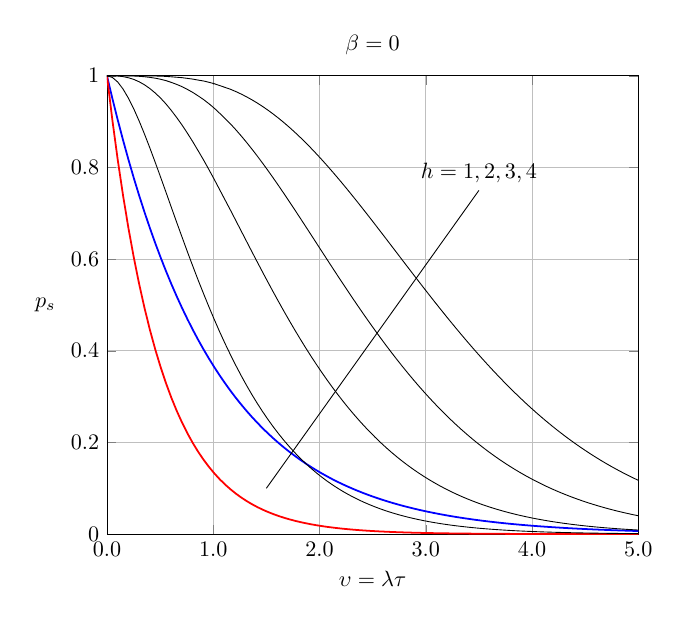
\begin{tikzpicture}[scale=0.8]

\begin{axis}
[
  title={$\beta = 0$},
%   width  = 0.8*\columnwidth, 
%   height = 0.4*\columnwidth,
  legend style={at={(0.95,0.95)}, anchor=north east},
%   xmode=log,
  xlabel={$\upsilon=\lambda\tau$},
  ylabel={$p_s$}, ylabel style={rotate=-90},
%  yticklabel=\pgfmathprintnumber{\tick}\\ \%,
  xmin = 0, 	
  xmax = 5,
  ymin = 0, 	
  ymax = 1,
  x tick label style={
        /pgf/number format/.cd,
        fixed,
        fixed zerofill,
        precision=1,
        /tikz/.cd
  },
  grid = both,
  scale only axis,
]
% 	\legend{slotted ALOHA, unslotted ALOHA}
    
    \addplot[thick, blue, domain = 0:5, samples=100] {exp(-x)};
    \addplot[thick, red, domain = 0:5, samples=100] {exp(-2*x)};
    
    \addplot[domain = 0:5, samples=100] {(1+2*x+x^2/2)*exp(-2*x)};
    \addplot[domain = 0:5, samples=100] {(1+2*x+2*x^2+(2/3)*x^3+x^4/12)*exp(-2*x)};
    \addplot[domain = 0:5, samples=100] {(1+2*x+2*x^2+(4/3)*x^3+(11/24)*x^4+x^5/12+x^6/144)*exp(-2*x)};
    \addplot[domain = 0:5, samples=100] {(1+2*x+2*x^2+(4/3)*x^3+(2/3)*x^4+(13/60)*x^5+(2/45)*x^6+x^7/180+x^8/2880)*exp(-2*x)};
    
%     \addplot[thick] table
%     [
% 		x expr = \thisrow{lam},
%     	y expr = \thisrow{25dB}
%     ] {./Data/envelopes.dat};

    \draw[-\arrowhead] (axis cs: 1.5,0.1) -- (axis cs: 3.50,0.75) node[anchor=south] 
        {$h = 1, 2, 3, 4$};
\end{axis}

\end{tikzpicture}
